
\documentclass[thmcnt=section, color=blue, 12pt]{my-elegantbook}

% Index page
\usepackage{imakeidx}
\makeindex[columns=2, intoc, options=-s index_style.ist]

% Title and author
\title{Mathematical Analysis}
\author{Isaac FEI}

% Reference file
\addbibresource{mathematical-analysis.bib} 

% Image of the book cover
\cover{cover}

\begin{document}

% Print title and cover page
\maketitle

%--------
% Preface
%--------

\frontmatter
\chapter*{Preface}

This book mainly follows the structure of \cite{apostolMathematicalAnalysisModern1974}.

%------------------------------

% Print table of contents
\tableofcontents
\mainmatter

%-------------------------------
% Main document starts from here
%-------------------------------

%==============================

\chapter{Point-Set Topology}

%==============================

\chapter{Functions of Bounded Variation and Rectifiable Curves}

%------------------------------ 

\section{Functions of Bounded Variation}

\begin{definition}
	Let $[a, b]$ be an interval.
	A set of points
	\begin{align*}
		P = \{ x_0, x_1, \dots, x_n \}
	\end{align*}
	satisfying
	\begin{align*}
		a = x_0 < x_1 < \cdots < x_n = b
	\end{align*}
	is called a \textbf{partition}\index{partition of an interval} of $[a, b]$.

	The interval $[x_{k-1}, x_k]$ is called the $k$-th subinterval of $P$,
	and we oftern write $\Delta x_k = x_k - x_{k-1}$.

	The collection of all partitions of $[a, b]$ is denoted by $\CALP [a, b]$.
\end{definition}


\begin{note}
	In mathematics texts, we have another definition of partitions,
	which states that a partition of a set $S$ is a collection of subsets of $S$
	such that they are disjoint and their union equals $S$.
	We should not confuse these two definitions.
\end{note}

\begin{definition}
	Let $f$ be a real-valued function on $[a, b]$.
	If $P = \{x_0, \dots x_n\}$ is a partition of $[a, b]$,
	write $\Delta f_k = f(x_k) - f(x_{k-1})$.
	If there exists a positive number $M$ such that
	\begin{align}
		\sum_{k=1}^n \abs{\Delta f_k} \leq M \label{eq:1}
	\end{align}
	for all partitions $P$ of $[a, b]$, then we say that $f$
	is \textbf{of bounded variation}\index{functions of bounded variation}
	on $[a, b]$.
\end{definition}

A simple observation is that a function of bounded variation is also bounded.

\begin{proposition} \label{prop:2}
	Let $f$ be a function of bounded variation on $[a, b]$.
	Then $f$ is bounded on $[a, b]$.
\end{proposition}

\begin{proof}
	By definition, there exists $M > 0$ such that \eqref{eq:1} holds
	for any partitions of $[a, b]$.
	For any $x \in (a, b)$, consider the partition $P = \{a, x, b\}$.
	We have
	\begin{align*}
		\abs{f(x) - f(a)} + \abs{f(b) - f(x)} \leq M
	\end{align*}
	This implies that $\abs{f(x) - f(a)} \leq M$, which further
	implies $\abs{f(x)} \leq \abs{f(a)} + M$.
	Note that $x$ is arbitrarily chosen from $(a, b)$.
	Therefore, $f$ is indeed bounded on $[a, b]$.
\end{proof}

But a bounded function is not necessarily of bounded variation.

\begin{example} \label{eg:1}
	Consider the function
	\begin{align*}
		f(x) = \begin{cases}
			       \cos \frac{1}{x}, & x \in (0, 1] \\
			       0,                & x = 0
		       \end{cases}
	\end{align*}
	Its graph is shown in Figure~\ref{fig:1}.
	\begin{figure}[H]
		\centering
		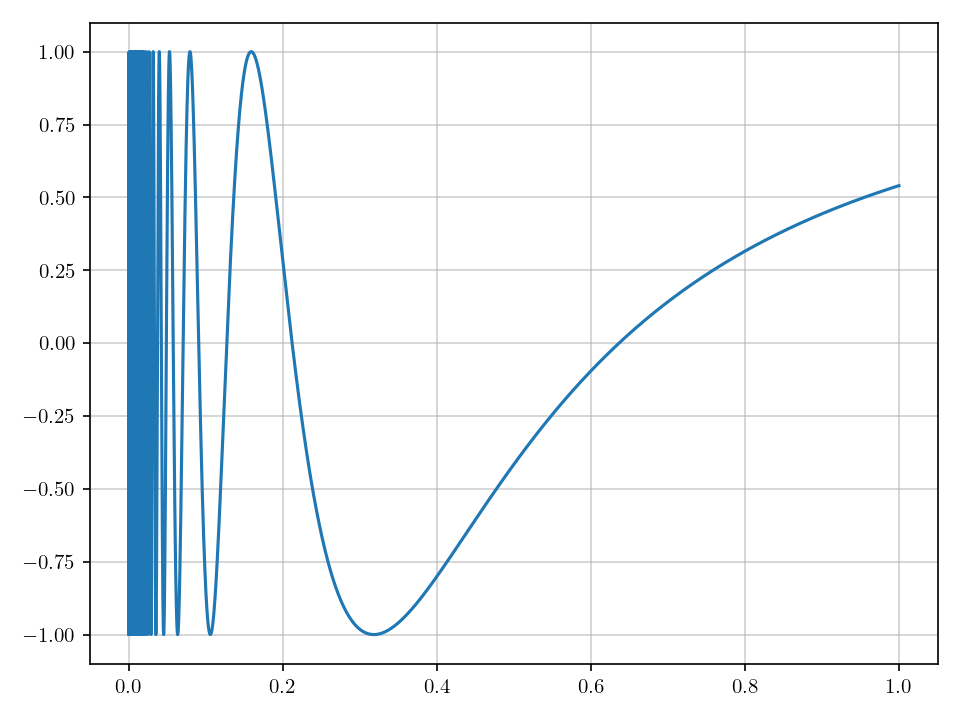
\includegraphics[width=0.6\textwidth]{figures/bounded-function-that-is-not-of-bounded-variation.png}
		\caption{Graph of the function $f(x) = \cos\frac{1}{x}$ for $x \in (0, 1]$ and $f(0) = 0$. It is bounded on $[0, 1]$ but not of bounded variation for it varias rapidly near $x=0$.}
		\label{fig:1}
	\end{figure}
	Clearly, this function is bounded by $1$.
	But intuitively, it is not of bounded variation since it varies rapidly
	near $x=0$.
	Let $P$ be a partition of $[0, 1]$ where each $x_k$ is given by
	\begin{align*}
		x_k = \begin{cases}
			      \frac{1}{(n-k) \pi}, & 1 \leq k \leq n-1 \\
			      0,                   & k = 0             \\
			      1,                   & k = n
		      \end{cases}
	\end{align*}
	For $k=1, \dots, n-1$, we have
	\begin{align*}
		f(x_k) = \cos ( (n-k) \pi ) \in \{-1, 1\}
	\end{align*}
	The function value is either $1$ or $-1$ and the sign alternates between
	each two consecutive points. Hence,
	\begin{align*}
		\sum_{k=1}^{n} \abs{\Delta f_k}
		\geq \sum_{k=2}^{n-1} \abs{\Delta f_k} = 2 (n - 2)
	\end{align*}
	As we increase the number of points in the partition, $\sum \abs{\Delta f_k}$
	will exceeds any given number.
	Therefore, $f$ is not of bounded variation on $[0, 1]$.
\end{example}

\begin{proposition} \label{prop:1}
	If $f$ is monotonic on $[a, b]$, then $f$ is of bounded variation on $[a, b]$.
\end{proposition}

\begin{proof}
	Assume $f$ is increasing.
	For any partition $P = \{x_0, \dots, x_n\}$ of $[a, b]$, we have
	\begin{align*}
		\sum_{k=1}^n \abs{\Delta f_k}
		= \sum_{k=1}^n (f(x_k) - f(x_{k-1}))
		= f(b) - f(a)
	\end{align*}
	Therefore, $f$ is of bounded variation on $[a, b]$.

	If $f$ is decreasing, then $-f$ is increasing.
	Applying what we have proved, we may conclude that $-f$ is of bounded variation.
	Hence, $f$ is also of bounded variation
	since $\sum \abs{\Delta (-f)_k} = \sum \abs{\Delta f_k}$.
\end{proof}

\begin{proposition} \label{prop:3}
	Suppose that $f$ is continuous on $[a, b]$ and the
	derivative $f^\prime$ exists in $(a, b)$.
	If $\abs{f^\prime(x)} \leq A$ for all $x \in (a, b)$,
	then $f$ is of bounded variation on $[a, b]$.
\end{proposition}

\begin{note}
	The assumption that $f$ being continuous on $[a, b]$,
	and $f^\prime$ exists in $(a, b)$ coincides with the mean value theorem.
	And indeed, it is the key of this proof.
\end{note}

\begin{proof}
	Let $P = \{x_0, \dots, x_n\}$ be a partition of $[a, b]$.
	By the mean value theorem, there exists $t_k \in (x_{k-1}, x_k)$
	for all $k=1, \dots, n$ such that
	\begin{align*}
		f(x_k) - f(x_{k-1}) = f^\prime(t_k) (x_k - x_{k-1})
	\end{align*}
	It then follows that
	\begin{align*}
		\sum_{k=1}^n \abs{\Delta f_k}
		 & = \sum_{k=1}^n \abs{f^\prime(t_k)} (x_k - x_{k-1}) \\
		 & \leq \sum_{k=1}^n A (x_k - x_{k-1})                \\
		 & = A (f(b) - f(a))
	\end{align*}
	Therefore, $f$ is of bounded variation on $[a, b]$.
\end{proof}

The following is a well crafted example of showing that
a continuous and differentiable function is not necessarily
of bounded variation
if we do not impose that its derivative is bounded in the interior.

\begin{example}
	Consider function defined on $[0, 1]$ given by
	\begin{align*}
		f(x) = \begin{cases}
			       x \cos \frac{\pi}{2x}, & x \in (0, 1] \\
			       0,                     & x = 0
		       \end{cases}
	\end{align*}
	Its graph is shown in Figure \ref{fig:2}.

	\begin{figure}[H]
		\centering
		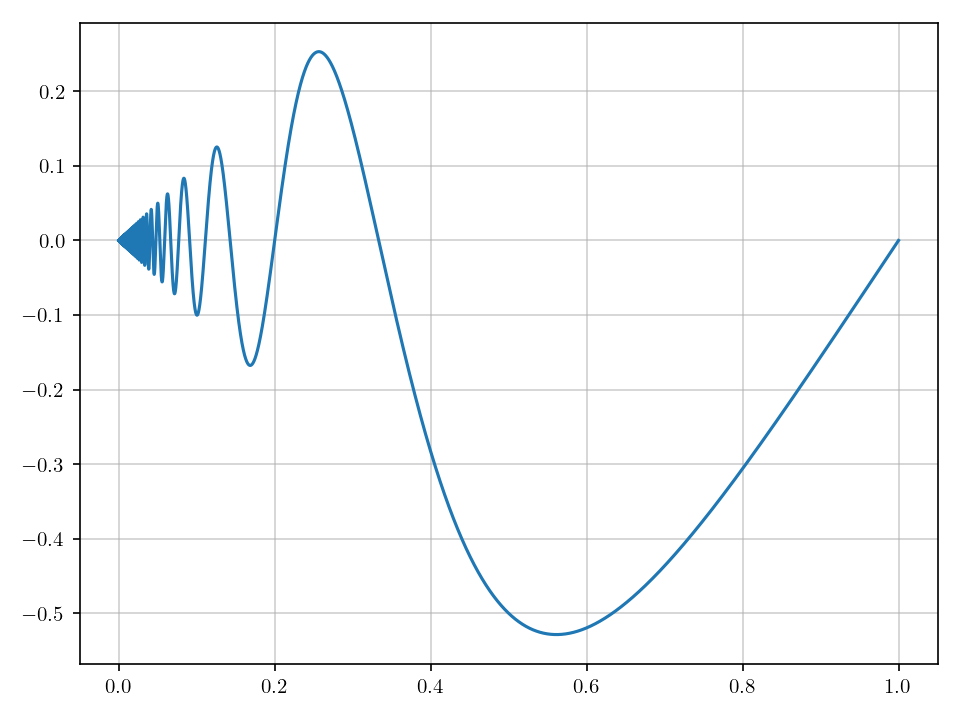
\includegraphics[width=0.6\textwidth]{figures/continuous-function-that-is-not-of-bounded-variation.png}
		\caption{Graph of the function $f(x) = x \cos \frac{\pi}{2x}$ for $x \in (0, 1]$ and $f(0) = 0$. This function is continuous and its derivative exists in $(0, 1)$. But the derivative is unbounded.}
		\label{fig:2}
	\end{figure}

	The fact that this function is not of bounded variation may be less intuitive
	than the one given in Example~\ref{eg:1}.
	The fucntion still varies rapidly near $x=0$.
	However, it does not range from $-1$ and $1$.
	Instead, it damps out at $x=0$ and becomes $0$.
	But we will show in the following that we can find a partition so fine that
	by collecting each small function variation,
	the overall sum may still increase to infinity.

	Consider the partition
	\begin{align*}
		P = \{0, \frac{1}{2n}, \frac{1}{2n - 1}, \dots, \frac{1}{3}, \frac{1}{2}, 1\}
	\end{align*}
	We have
	\begin{align*}
		\sum_k \abs{\Delta f_k}
		 & = \frac{1}{2n} + \frac{1}{2n} + \frac{1}{2n - 1} + \frac{1}{2n - 1}
		+ \dots + \frac{1}{2} + \frac{1}{2}                                    \\
		 & = 1 + \cdots + \frac{1}{n}
	\end{align*}
	As $n$ gets larger and larger,
	the sum on the right hand-side will increase infinitely
	for we know that the harmonic series $\sum \frac{1}{n}$ diverges.
	Therefore, this function is not of bounded variation.
\end{example}

Of course, the condition of the derivative being bounded is not necessary
for a function to be of bounded variation.

\begin{example}
	The derivative of the squre root function $f(x) = \sqrt{x}$ in $(0, 1)$
	is $f^\prime(x) = \frac{1}{2\sqrt{x}}$,
	which tends to infinity as $x \to 0$.
	But $f$ is clearly of bounded variation on $[0, 1]$
	by Proposition~\ref{prop:1} for it is increasing.
\end{example}

%------------------------------ 

\section{Total Variation}

Recall that $f$ is said to be of bounded of variation
on $[a, b]$ if, equivalently to what we stated, the set
\begin{align}
	\set{\sum_{k=1}^n \abs{\Delta f_k}}{P \in \CALP [a, b]}
	\label{eq:2}
\end{align}
is bounded above.
This set is of course nonempty for $\{a, b\}$ is clearly a partition.
By the least upper bound property,
the set in \eqref{eq:2} has a supremum, which is referred to as
\textbf{total variation}\index{total variation} of $f$ on $[a, b]$.

\begin{definition}
	Let $f$ be of bounded variation on $[a, b]$.
	The total variation, denoted by $V_a^b (f)$,
	of $f$ on $[a, b]$ is defined as
	\begin{align*}
		V_a^b (f) := \sup \set{\sum_{k=1}^n \abs{\Delta f_k}}{P \in \CALP [a, b]}
	\end{align*}
\end{definition}

\begin{note}
	We adopt the notation $V_a^b(f)$,
	which is inspired by the notion of
	a definite integral $\int_a^b f(x) \dif x$.
	And as we shall see,
	these two concepts indeed share some similar properties, namely,
	the linear properties.

	Notations are very important for they provide intuitive expressions
	of the intrinsic mathematical concepts.
\end{note}

From this definition,
we have some simple observations.
First, the value of $V_a^b (f)$ is nonnegative.
And it is easy to prove that $V_a^b (f) = 0$
if and only if $f$ is constant on $[a, b]$.

\begin{theorem} \label{thm:1}
	Let $f$ and $g$ be of bounded variation on $[a, b]$, then
	so are their sum, difference and product.
	Moreover, we have the following inequalities:
	\begin{align}
		V_a^b (f \pm g)  \leq V_a^b (f) + V_a^b (g)
		\label{eq:3}
	\end{align}
	and
	\begin{align}
		V_a^b (fg)       \leq \sup_{x \in [a, b]} \abs{g(x)} V_a^b (f)
		+ \sup_{x \in [a, b]} \abs{f(x)} V_a^b (g)
		\label{eq:4}
	\end{align}
\end{theorem}

\begin{note}
	Note that the supremums in \eqref{eq:4} indeed exist
	since the functions $f$ and $g$ are bounded due to Proposition~\ref{prop:2}.
\end{note}



\begin{proof}
	We first show that the sum and the difference of two functions
	are of bounded variation, and satisfy \eqref{eq:3}.
	Let $P$ be an arbitrary partition of $[a, b]$.
	On each subinterval, we have
	\begin{align*}
		\abs{\Delta (f \pm g)_k}
		 & = \abs{f(x_{k}) \pm g(x_{k}) - [f(x_{k-1}) \pm g(x_{k-1})]} \\
		 & = \abs{\Delta f_k \pm \Delta g_k}                           \\
		 & \leq \abs{\Delta f_k} + \abs{\Delta g_k}
	\end{align*}
	Taking the sum over $k$, we have
	\begin{align*}
		\sum_{k} \abs{\Delta (f \pm g)_k}
		\leq \sum_{k} \abs{\Delta f_k} + \sum_k \abs{\Delta g_k}
		\leq V_a^b (f) + V_a^b (g)
	\end{align*}
	The above inequality shows that $f \pm g$ is of bounded variation on $[a, b]$,
	and \eqref{eq:3} is satisfied.

	In the following, we show that the product of two Functions
	are of bounded variation and satisfies \eqref{eq:4}.
	Let $P$ be an arbitrary partition of $[a, b]$.
	On each subinterval, we have
	\begin{align*}
		\abs{\Delta (fg)_k}
		 & = \abs{f(x_{k}) g(x_{k}) - f(x_{k-1}) g(x_{k-1})}                                \\
		 & \text{Add and subtract the term $f(x_{k-1})g(x_{k})$}                            \\
		 & = \abs{ g(x_{k})[ f(x_{k}) - f(x_{k-1})] + f(x_{k-1})[ g(x_{k}) - g(x_{k-1}) ] } \\
		 & \leq \abs{g(x_{k})} \abs{\Delta f_k} + \abs{f(x_{k-1})} \abs{ \Delta g_k }       \\
		 & \leq \sup_{x \in [a, b]} \abs{g(x)} \abs{\Delta f_k}
		+ \sup_{x \in [a, b]} \abs{f(x)} \abs{\Delta g_k}
	\end{align*}
	Summing over $k$, we have
	\begin{align*}
		\sum_k \abs{\Delta (fg)_k}
		\leq \sup_{x \in [a, b]} \abs{g(x)} \sum_k \abs{\Delta f_k}
		+ \sup_{x \in [a, b]} \abs{f(x)} \sum_k \abs{\Delta g_k} \\
		\leq  \sup_{x \in [a, b]} \abs{g(x)} V_a^b (f)
		+ \sup_{x \in [a, b]} \abs{f(x)} V_a^b (g)
	\end{align*}
	This shows the product $fg$ is in fact of bounded variation on $[a, b]$,
	and \eqref{eq:4} is satisfied.
\end{proof}

We must exclude the quotients from the above theorem
since the reciprocal $\frac{1}{f}$ of $f$ may not be of bounded variation
even though $f$ is.

\begin{example}
	Consider function
	\begin{align*}
		f(x) = \begin{cases}
			       1-x, & 0 \leq x < 1     \\
			       -x,  & 1 \leq x  \leq 2
		       \end{cases}
	\end{align*}
	Function $f$ is of bounded variation on $[0, 2]$ since it is decreasing.
	Its reciprocal is
	\begin{align*}
		\frac{1}{f(x)} = \begin{cases}
			                 \frac{1}{1-x}, & 0 \leq x < 1     \\
			                 -\frac{1}{x},  & 1 \leq x  \leq 2
		                 \end{cases}
	\end{align*}
	Figure \ref{fig:3} depicts the graphs of $f$ and $\frac{1}{f}$.
	\begin{figure}[H]
		\centering
		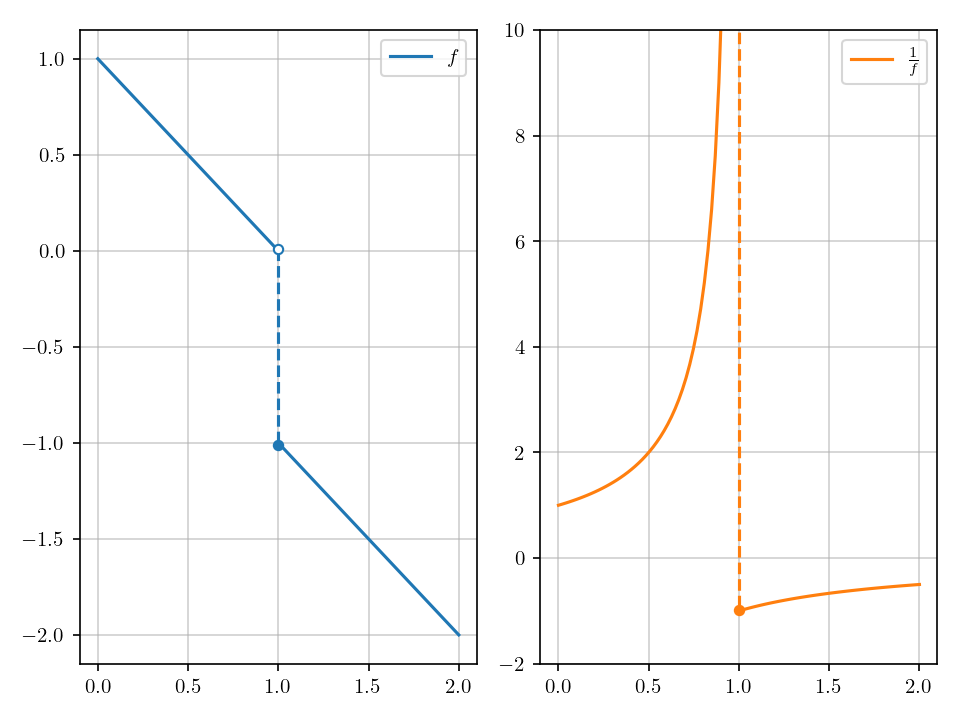
\includegraphics[width=0.6\textwidth]{figures/reciprocal-not-of-bounded-variation.png}
		\caption{Left: $f$ is of bounded variation for it is decreasing. Right: $\frac{1}{f}$ is not of bounded variation for it is unbounded.}
		\label{fig:3}
	\end{figure}
	Note that $\frac{1}{f}$ goes to positive infinity when $x \to 1^-$.
	Therefore, by Proposition~\ref{prop:2}, $\frac{1}{f}$ is not of bounded variation on $[0, 2]$
	since it is not bounded.
\end{example}

To extend Theorem~\ref{thm:1} to quotients,
we need to required that $f$ is bounded away from zero in the interval.

\begin{theorem}
	Let $f$ be of bounded variation on $[a, b]$.
	And there exists $m > 0$ such that $f(x) \geq m$ for all $x \in [a, b]$.
	Then the reciprocal of $f$ is of bounded variation on $[a, b]$, and
	\begin{align*}
		V_a^b ( \frac{1}{f} )
		\leq \frac{1}{m^2} V_a^b (f)
	\end{align*}
\end{theorem}

\begin{proof}
	Let $P$ be any partition of $[a, b]$.
	On each subinterval $[x_{k-1}, x_k]$, we have
	\begin{align*}
		\abs{\Delta (\frac{1}{f})_k}
		 & = \abs{\frac{1}{f(x_k)} - \frac{1}{f(x_{k-1})}} \\
		 & = \abs{\frac{\Delta f_k}{f(x_{k-1}) f(x_k)}}    \\
		 & \leq \frac{\abs{ \Delta f_k }}{m^2}
	\end{align*}
	Summing over $k$, we have
	\begin{align*}
		\sum_k \abs{\Delta (\frac{1}{f})_k}
		\leq \frac{1}{m^2} \sum_k \abs{\Delta f_k}
		\leq \frac{1}{m^2} V_a^b (f)
	\end{align*}
	Therefore, $\frac{1}{f}$ is of bounded variation on $[a, b]$.
\end{proof}

\subsection{Additive Property of Total Variation}

Consider the following continuous function defined on $[0, 3]$:
\begin{align*}
	f(x) = \begin{cases}
		       x,           & 0 \leq x \leq 1 \\
		       -(x-1)(x-3), & 1 < x \leq 3
	       \end{cases}
\end{align*}
Figure~\ref{fig:4} depicts its graph.
\begin{figure}[H]
	\centering
	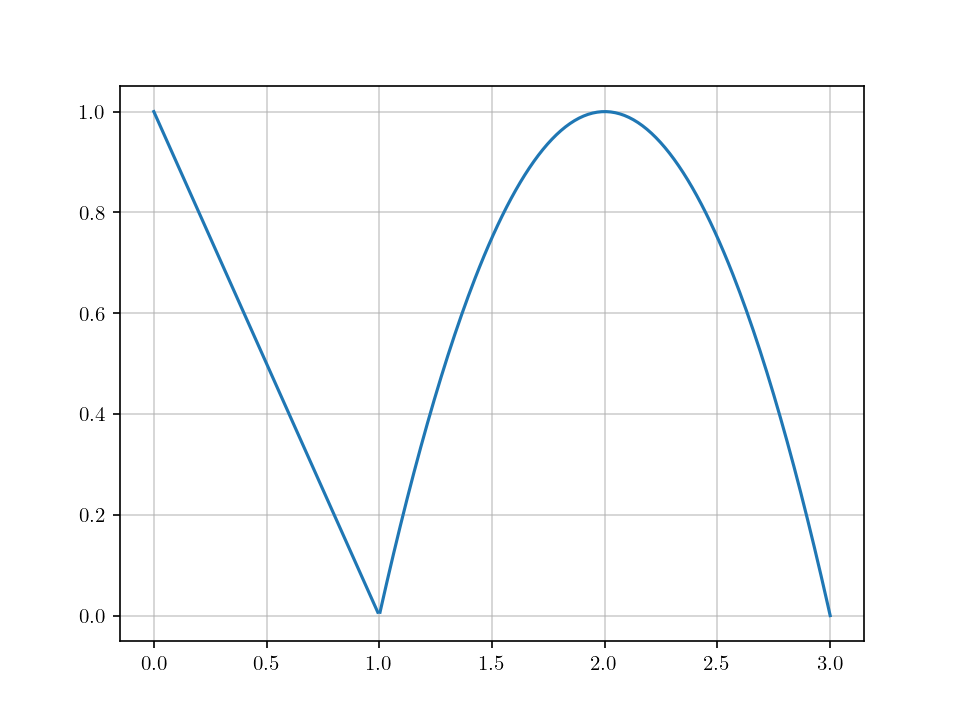
\includegraphics[width=0.6\textwidth]{figures/additive-property-of-total-variation-example-1.png}
	\caption{Function $f$ is of bounded variation on $[0, 1]$ and $[1, 3]$, separately.}
	\label{fig:4}
\end{figure}
We cannot prove $f$ is of bounded of variation using
Proposition~\ref{prop:3} since its derivative does not exist at $x=1$.
However, we note that $f$ is of bounded variation
on $[0, 1]$ and $[1, 3]$, separately.
And intuitively, having only
fintely many points at which $f^\prime$ fail to exist
should not
prevent $f$ from being of bounded of variation on the entire interval.
This is indeed true, which is stated in the following theorem.

\begin{theorem}
	Let $f$ be of bounded variation on $[a, b]$, and $c \in (a, b)$.
	Then $f$ is of bounded variation on the subintervals $[c, b]$ and $[a, c]$.
	Moreover, we have
	\begin{align}
		V_a^b(f) = V_a^c(f) + V_c^b(f)
		\label{eq:9}
	\end{align}
\end{theorem}

\begin{proof}
	We will first show that $f$ is of bounded variation on each subinterval, and
	\begin{align}
		V_a^c(f) + V_c^b(f) \leq V_a^b(f)
		\label{eq:5}
	\end{align}
	To make the proof clear,
	we introduce the notation $S(P) = \sum_k \abs{\Delta f_k}$
	where $P$ is any partition of an arbitrary subinterval contained in $[a, b]$.
	(Though it suffices to just consider the subintervals $[a, b]$, $[a, c]$
	and $[c, b]$ in this proof.)

	Let $P^\prime$ and $P^{\prime\prime}$ be partitions of $[a, c]$ and $[c, b]$,
	respectively,
	and let $P = P^\prime \cup P^{\prime\prime}$.
	Note that $P$ is a partition of $[a, b]$,
	and by reviewing the notation of $S(P)$
	one may easily conclude that $S(P^\prime) + S(P^{\prime\prime}) = S(P)$.
	Since $f$ is of bounded of variation on $[a, b]$, we have
	\begin{align}
		S(P^\prime) + S(P^{\prime\prime}) = S(P) \leq V_a^b (f)
		\label{eq:6}
	\end{align}
	The above inequality holds for any partition $p^\prime$ of $[a, c]$
	and any partition $p^{\prime\prime}$ of $[c, b]$.
	Therefore, by definition, $f$ is of bounded variation on $[a, c]$ and $[c, b]$.
	Moreover, taking the supremum over $P^\prime$ and then over $P^{\prime\prime}$
	on both sides of \eqref{eq:6}, we will obtain extactly \eqref{eq:5}.

	To show the equality \eqref{eq:9}, we also need to show
	\begin{align}
		V_a^c(f) + V_c^b(f) \geq V_a^b (f)
		\label{eq:7}
	\end{align}
	Let $\varepsilon > 0$ be arbitrary.
	There exists a partition $P$ of $[a, b]$
	such that $S(P) > V_a^b(f) - \varepsilon$.
	Let
	\begin{align*}
		P^\prime = ( P \cap [a, c] ) \cup \{c\} \quad \text{and} \quad
		P^{\prime\prime} = ( P \cap [c, b] ) \cup \{c\}
	\end{align*}
	It is clear that $P^\prime$ and $P^{\prime\prime}$
	are partitions of $[a, c]$ and $[c, b]$, respectively.
	If $c \in P$, then clearly $S(P) = S(P^\prime) + S(P^{\prime\prime})$.
	If $c \notin P$, supposing the intermediate
	subinterval of $P$ containing $c$ is $[x_{j-1}, x_j]$,
	then we have
	\begin{align*}
		\abs{\Delta f_j} = \abs{f(x_j) - f(x_{j-1})}
		\leq \abs{f(x_j) - f(c)} + \abs{f(c) -  f(x_j)}
	\end{align*}
	It then follows that $S(P) \leq S(P^\prime) + S(P^{\prime\prime})$.
	Hence, no matter if $c \in P$ or $c \notin P$, we have
	\begin{align}
		V_a^c(f) + V_c^b(f) \geq S(P^\prime) + S(P^{\prime\prime}) \geq S(P) > V_a^b(f) - \varepsilon
		\label{eq:8}
	\end{align}
	Because \eqref{eq:8} holds for every $\varepsilon > 0$, \eqref{eq:7} is proved.
\end{proof}


%==============================

% References
\printbibliography[heading=bibintoc, title=References]

%==============================

% Print index page
\printindex

\end{document}
